%%%%%%%%%%%%%%%%%%%%%%%%%%%%%%%%%%%%%%%%%%%%%%%%%%%%%%%%%%%%%%%%%%%%%%
% How to use writeLaTeX: 
%
% You edit the source code here on the left, and the preview on the
% right shows you the result within a few seconds.
%
% Bookmark this page and share the URL with your co-authors. They can
% edit at the same time!
%
% You can upload figures, bibliographies, custom classes and
% styles using the files menu.
%
%%%%%%%%%%%%%%%%%%%%%%%%%%%%%%%%%%%%%%%%%%%%%%%%%%%%%%%%%%%%%%%%%%%%%%

\documentclass[12pt]{article}

\usepackage{sbc-template}

\usepackage{graphicx,url}

%\usepackage[brazil]{babel}   
\usepackage[utf8]{inputenc} 

\usepackage{float}
\usepackage{hyperref}

\usepackage{listings}
\usepackage{color}

\definecolor{dkgreen}{rgb}{0,0.6,0}
\definecolor{gray}{rgb}{0.5,0.5,0.5}
\definecolor{mauve}{rgb}{0.58,0,0.82}

\lstset{frame=none,
  language=C++,
  aboveskip=3mm,
  belowskip=3mm,
  showstringspaces=false,
  columns=flexible,
  basicstyle={\small\ttfamily},
  numbers=none,
  numberstyle=\tiny\color{gray},
  keywordstyle=\color{blue},
  commentstyle=\color{dkgreen},
  stringstyle=\color{mauve},
  breaklines=true,
  breakatwhitespace=true,
  tabsize=3
}

     
\sloppy

\title{EspNow}

\author{Fabricio Araújo Dias}

\address{Instituto Federal de Educação, Ciência e Tecnologia do Ceará
  (IFCE)\\
  Avenida Vice-Presidente José Alencar, S/N -- 61.939-140 -- Maracanaú -- CE -- Brasil
  \email{fabricio.araujo61@aluno.ifce.edu.br}
}

\begin{document} 

\maketitle

\begin{abstract}
    This report describes the step-by-step execution of the ninth practical activity in the microcontrollers course, which focuses on using the ESP-NOW protocol to send messages between two ESP32s. To test the sending, a small test was carried out to define the color of an RGB LED.
\end{abstract}
     
\begin{resumo} 
    Esse relatório descreve o passo a passo da realização da nona atividade prática da disciplina de microcontroladores que se foca no uso do protocolo ESP-NOW para envio de mensagens entre dois ESP32. Para testar o envio, foi feito um pequeno teste para definir a cor de um LED RGB.
\end{resumo}

\section{Introdução}

A nona atividade prática da disciplina de Microcontroladores consiste em fazer exatamente a mesma coisa feita na aula passada, que era sobre o protocolo MQTT, mas agora utilizando o protocolo ESP-NOW, que é um protocolo que se destaca por ter sido produzido pela Espressif, a desenvolvedora do ESP32. 

O protocolo ESP-NOW também é um protocolo de envio de mensagens que permite a comunicação de ESP32s sem a utilização de uma rede Wi-Fi. Bastando apenas que os dispositivos estejam pareados.

Para testar o envio e o recebimento de mensagens, iremos desenvolver um código para que imprima a mensagem no monitor e que defina a cor de um LED RGB.

\section{Configuração no ESP32}

Utilizamos um ESP32 de 30 pinos, uma \textit{protoboard} de 400 pontos, um LED RGB, três resistores de 390 \textit{ohms} cada, quatro cabos macho-fêmea e um cabo \textit{microUSB}.

Primeiro, dispomos o LED RGB na parte lateral da protoboard para que possamos colocar o cátodo do LED na linha negativa e os demais terminais em pontos qualquer. Em cada terminal do LED, colocamos um resistor de 390 ohms, para evitar o risco do LED queimar.

\begin{figure}[H]
    \centering
    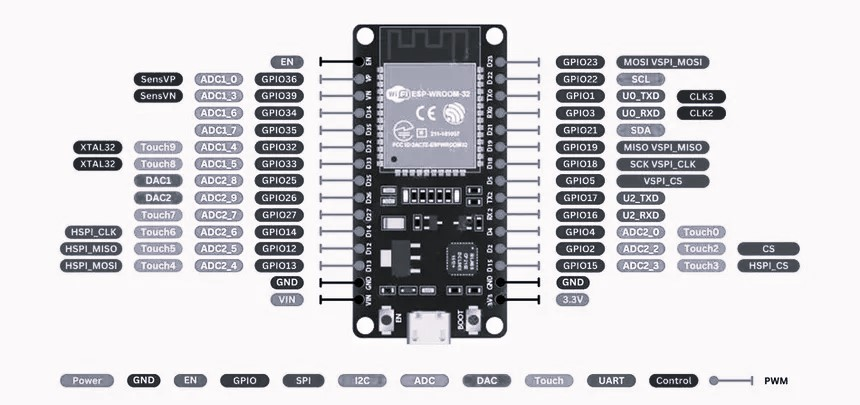
\includegraphics[width=0.5\linewidth]{img/esp32_pinout.png}
    \caption{Pinout do ESP32.}
    \label{fig:esp32-pinout}
\end{figure}

Para terminar, vamos conectar os pinos do ESP32 à \textit{protoboard}. Escolhemos os pinos 18, 19 e 21 para o terminal vermelho, verde e azul do LED RGB, respectivamente. Utilizamos três cabos macho-fêmea para conectar os pinos aos pontos que estão conectados ao terminal do resistores. Usamos o último cabo para conectar o GND do ESP32 à linha negativa da \textit{protoboard}, onde está conectado o terminal do cátodo do LED RGB.

\begin{figure}[H]
    \centering
    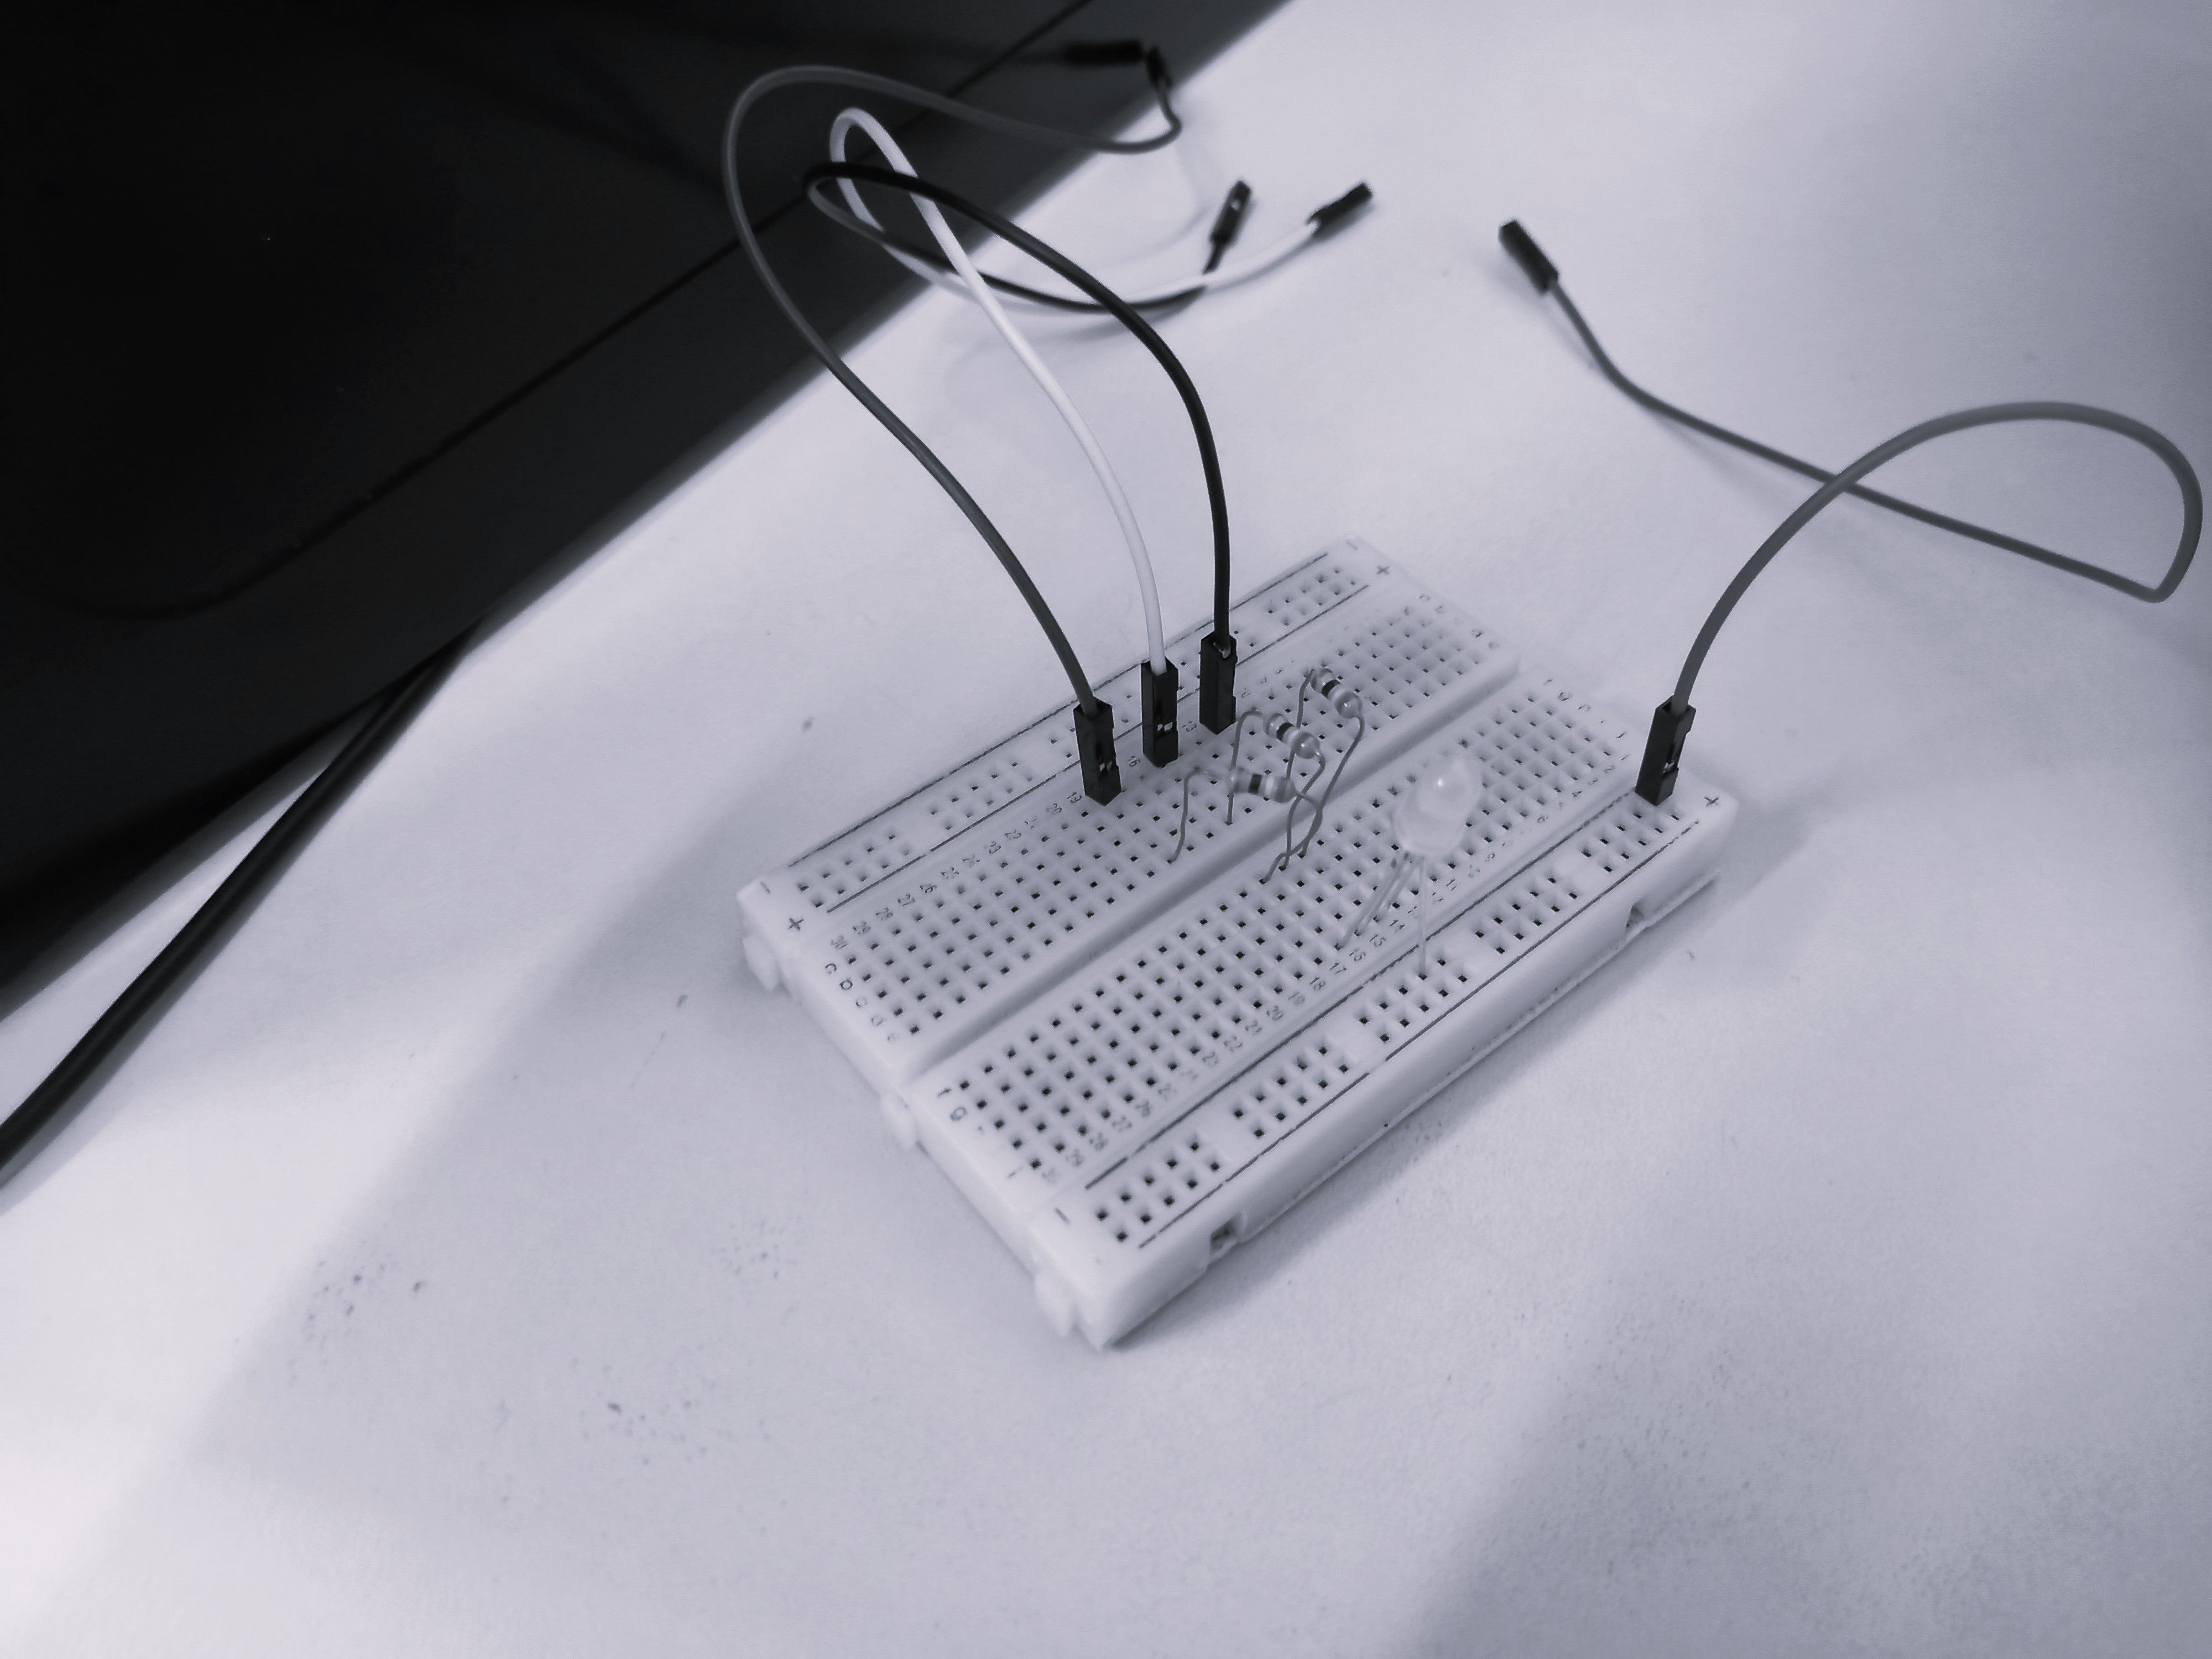
\includegraphics[width=0.5\linewidth]{img/20241125_095139.jpg}
    \caption{Configuração final.}
    \label{fig:final-config}
\end{figure}

\section{Desenvolvimento do Código}

Usamos novamente o Visual Studio Code junto com a extensão do PlatformIO. Na página inicial, criamos um novo projeto dando o nome de \textit{esp\_now\_}, declarando que a placa é \textit{Espressif ESP32 Dev Module} e utilizando o framework Arduino.

Uma pequena parte do código reutiliza o código de outras aulas que é referente ao LED RGB. Definimos constantes e configuramos eles para o modo de saída.

Por padrão, também definimos a taxa do monitor para 9600 e iniciamos o Serial.

\begin{lstlisting}
// platformio.ini
monitor_speed = 9600

// main.cpp
#define RED 18
#define GREEN 19
#define BLUE 21

void setup() {
    Serial.begin(9600);

    pinMode(RED, OUTPUT);
    pinMode(GREEN, OUTPUT);
    pinMode(BLUE, OUTPUT);
}
\end{lstlisting}

\subsection{Descobrindo o endereço MAC do ESP32}

Foi necessário utilizar funções das bibliotecas \textit{WiFi} e \textit{esp\_wifi} para descobrir o endereço MAC do ESP32. São bibliotecas padrões e não precisam ser instaladas.

\begin{lstlisting}
#include <WiFi.h>
#include <esp_wifi.h
\end{lstlisting}

Em setup, configuramos o módulo \textit{WiFi} para que funcione em modo estacionário. Para então, chamarmos a função \textit{readMacAdress}.

\begin{lstlisting}
WiFi.mode(WIFI_STA);
readMacAddress();
\end{lstlisting}

A função não recebe parâmetros e nem tem retorno. Ela apenas imprime no monitor o endereço MAC. Criamos um vetor do tipo \textit{uint8\_t} chamada baseMac para guardar os seis campos do endereço MAC. Utilizando uma função chamada \textit{esp\_wifi\_get\_mac}, e passando como parâmetros a constante WIFI\_IF\_STA e o vetor \textit{baseMac}, todo o endereço será armazenado nas posições do vetor.

\begin{lstlisting}
void readMacAddress(){
    uint8_t baseMac[6];
    esp_err_t ret = esp_wifi_get_mac(WIFI_IF_STA, baseMac);
\end{lstlisting}

Essa função também retorna um valor do tipo \textit{esp\_err\_t} que diz se foi possível ler o endereço MAC ou não. Guardados numa variável chamada \textit{ret} e comparamos se ela é igual à \textit{ESP\_OK}, indicando que a leitura foi feita. Sendo positivo, imprimimos todas as posições desse vetor no monitor utilizando a função \textit{printf} do Serial para a impressão formatada. 

\begin{lstlisting}
if (ret == ESP_OK) {
    Serial.printf("%02x:%02x:%02x:%02x:%02x:%02x\n",
    baseMac[0], baseMac[1], baseMac[2],
    baseMac[3], baseMac[4], baseMac[5]);
\end{lstlisting}

Enviando o código para o ESP32, o endereço não apareceu de imediato no monitor. Apenas quando foi apertado o botão EN do microcontrolador que o endereço foi imprimido. Como essa parte do código não seria mais utilizada após isso, apagamos ela do código.

\subsection{ESP-NOW}

Para inicializar o ESP-NOW, começamos importando a biblioteca \textit{esp\_now} que também é padrão do ESP32 e não precisa ser instalada.

\begin{lstlisting}
#include <esp_now.h>
#include <WiFi.h>
\end{lstlisting}

Em setup, configuramos o módulo \textit{WiFi} no modo estacionário, que já foi feito na hora que estavamos descobrindo o endereço MAC do ESP32. 

\begin{lstlisting}
WiFi.mode(WIFI_STA);
\end{lstlisting}

Usamos a função esp\_now\_init() para inicializar o ESP-NOW. A função retorna um valor para indicar se a inicialização foi realizada ou não. Se ele retornar ESP\_OK, é que foi realizada. Caso seja diferente, interrompemos a execução por aí.

\begin{lstlisting}
if (esp_now_init() != ESP_OK) {
    Serial.println("Error initializing ESP-NOW");
    return;
}
\end{lstlisting}

Antes de desenvolver o envio e recebimento mensagens, definimos uma \textit{struct} para padronizar as mensagens. A \textit{struct} possui um vetor de caracteres, um inteiro, um \textit{float} e um \textit{booleano}. Logo em seguida, criamos uma variável chamada myData desse \textit{struct}.

\begin{lstlisting}
typedef struct struct_message {
    char a[32];
    int b;
    float c;
    bool d;
} struct_message;

struct_message myData;
\end{lstlisting}

\subsubsection{Preparando o recebimento de mensagens}

Criamos uma função chamada \textit{OnDataRecv} que é a função de \textit{callback} para o recebimento de mensagens. Como parâmetros, ela recebe um endereço MAC, a mensagem e o tamanho dela. 

\begin{lstlisting}
void OnDataRecv(const uint8_t * mac, const uint8_t *incomingData, int len) {
\end{lstlisting}

Para esse caso, vamos utilizar apenas a variável das mensagens. Ela vem no formato de uma variável constante do tipo \textit{uint8\_t}. Para visualzar essa mensagem, utilizamos a função \textit{memcpy} para copiar a mensagem que recebemos para a variável \textit{myData}. O tipo não é relevante, pois ele só copiar de um bloco de memória para outro, e isso permite que agora possamos acessar as informações da mensagem.

\begin{lstlisting}
memcpy(&myData, incomingData, sizeof(myData));
\end{lstlisting}

Podemos imprimir todos os dados da mensagem no monitor:

\begin{lstlisting}
Serial.print("Bytes received: ");
Serial.println(len);
Serial.print("Char: ");
Serial.println(myData.a);
Serial.print("Int: ");
Serial.println(myData.b);
Serial.print("Float: ");
Serial.println(myData.c);
Serial.print("Bool: ");
Serial.println(myData.d);
Serial.println();
\end{lstlisting}


Como foi dito na introdução, vamos testar esse envio de mensagens para definir a cor do LED RGB. Para isso, o conteúdo do vetor de caracteres deve ser "red", "green" ou "blue" para ter algum efeito. Usamos \textit{ifs} condicionais para configurar o nível dos pinos com a função \textit{digitalWrite}. Para realizar a comparação, é preciso converter o vetor de caracteres numa String.

\begin{lstlisting}
String color = String(myData.a);

if(color == "red") {
    digitalWrite(RED, HIGH);
    digitalWrite(GREEN, LOW);
    digitalWrite(BLUE, LOW);
} else if(color == "green") {
    digitalWrite(RED, LOW);
    digitalWrite(GREEN, HIGH);
    digitalWrite(BLUE, LOW);
} else if(color == "blue") {
    digitalWrite(RED, LOW);
    digitalWrite(GREEN, LOW);
    digitalWrite(BLUE, HIGH);
}
\end{lstlisting}

Para registrar essa função de callback, usamos a função \textit{esp\_now\_register\_recv\_cb}. O \textit{esp\_now\_recv\_cb\_t} é uma definição de tipo.

\begin{lstlisting}
esp_now_register_recv_cb(esp_now_recv_cb_t(OnDataRecv));
\end{lstlisting}

Assim, toda vez que o ESP32 receber mensagens, a função \textit{onDataRecv} será executada.

\subsubsection{Preparando o envio de mensagens}

Primeiro definimos o endereço MAC do outro ESP32 a qual queremos comunicar num vetor do tipo \textit{uint8\_t}. Lembrando que o endereço é dividido por campos no vetor. 

\begin{lstlisting}
uint8_t broadcastAddress[] = {0xFF, 0xFF, 0xFF, 0xFF, 0xFF, 0xFF};
\end{lstlisting}

Logo depois, criamos uma variável global do tipo \textit{esp\_now\_peer\_info\_t} chamada \textit{peerInfo} que guarda as informações sobre o outro dispositivo o qual queremos nos comunicar.

\begin{lstlisting}
esp_now_peer_info_t peerInfo;
\end{lstlisting}

Então, criamos uma função de \textit{callback} que será executada toda vez que enviamos uma mensagem. A função se chama \textit{OnDataSent} que recebe o endereço MAC do destinatário e o \textit{status} de envio. A função é bem simples. Ela só imprime no monitor se o envio da mensagem foi sucetivo ou não.

\begin{lstlisting}
void OnDataSent(const uint8_t *mac_addr, esp_now_send_status_t status) {
    Serial.print("\r\nLast Packet Send Status:\t");
    Serial.println(status == ESP_NOW_SEND_SUCCESS ? "Delivery Success" : "Delivery Fail");
}
\end{lstlisting}

Em setup, após inicializarmos o ESP-NOW, registramos a função \textit{OnDataSent} utilizando a função \textit{esp\_now\_register\_send\_cb}. O \textit{esp\_now\_send\_cb\_t} é para definição de tipos.

\begin{lstlisting}
esp_now_register_send_cb(esp_now_send_cb_t(OnDataSent));
\end{lstlisting}

Passamos para a parte de registrar o outro microcontrolador como par e enviar uma mensagem para ele. Vamos usar a variável \textit{peerInfo} que nada mais é que uma struct contendo as informações do outro dispositivo. Copiamos o endereço MAC para \textit{peer\_addr}, definimos o \textit{channel} (canal) como 0 para que ele use o canal onde a estação está ativada (por isso configuramos o módulo Wi-Fi para que seja estacionário), e que definimos \textit{false} em \textit{encrypted} para informar que a mensagem não está encriptada.

\begin{lstlisting}
memcpy(peerInfo.peer_addr, broadcastAddress, 6);
peerInfo.channel = 0;  
peerInfo.encrypt = false;
\end{lstlisting}

Agora, passamos o endereço de \textit{peerInfo} como parâmetro da função \textit{esp\_now\_add\_peer} para que ela registre o outro ESP32. A função retorna um valor para conferir se a operação deu certo ou não.

\begin{lstlisting}
if (esp_now_add_peer(&peerInfo) != ESP_OK){
    Serial.println("Failed to add peer");
    return;
}
\end{lstlisting}

Em \textit{loop}, enviamos a mensagem. Preenchemos os campos de \textit{myData}, sendo o mais importante o texto do vetor de caracteres que irá definir a cor do LED RGB. Para enviar a mensagem, usamos a função \textit{esp\_now\_send} que recebe o endereço do outro par, a mensagem e o tamanho. Fazemos \textit{casting} do endereço na memória de \textit{myData} para \textit{uint8\_t} e o tamanho da mensagem é o tamanho de \textit{myData}, que é o mesmo independente se todas as variáveis foram preenchidas ou não.

\begin{lstlisting}
strcpy(myData.a, "red");
myData.b = 3;
myData.c = 1.5;
myData.d = false;
\end{lstlisting}

A função \textit{esp\_now\_send} retorna um valor para indicar o status da operação. Se for bem sucedida, imprimimos que a mensagem foi enviada com sucesso. Se não, dizemos que o envio falhou. Colocamos um \textit{delay} de dois segundos para que o ESP32 não fique enviando a mensagem o tempo todo.

\begin{lstlisting}
esp_err_t result = esp_now_send(broadcastAddress, (uint8_t *) &myData, sizeof(myData));

if (result == ESP_OK) {
    Serial.println("Sent with success");
} else {
    Serial.println("Error sending the data");
}

delay(2000);
\end{lstlisting}

O código completo está disponível nesse \href{https://github.com/fabricio-araujo94/microcontroladores/tree/main/esp_now_}{repositório no GitHub}.

\section{Considerações Finais}

Por fim, conectamos o ESP32 ao computador utilizando o cabo \textit{microUSB} e enviamos o código para ele utilizando o comando \textit{Alt + Ctrl + U}. Assim, pedi para que o colega Pedro Emanuel enviasse mensagens para o meu ESP32, como "red" e "green", para alterar a cor do LED RGB.

\begin{figure}[H]
    \centering
    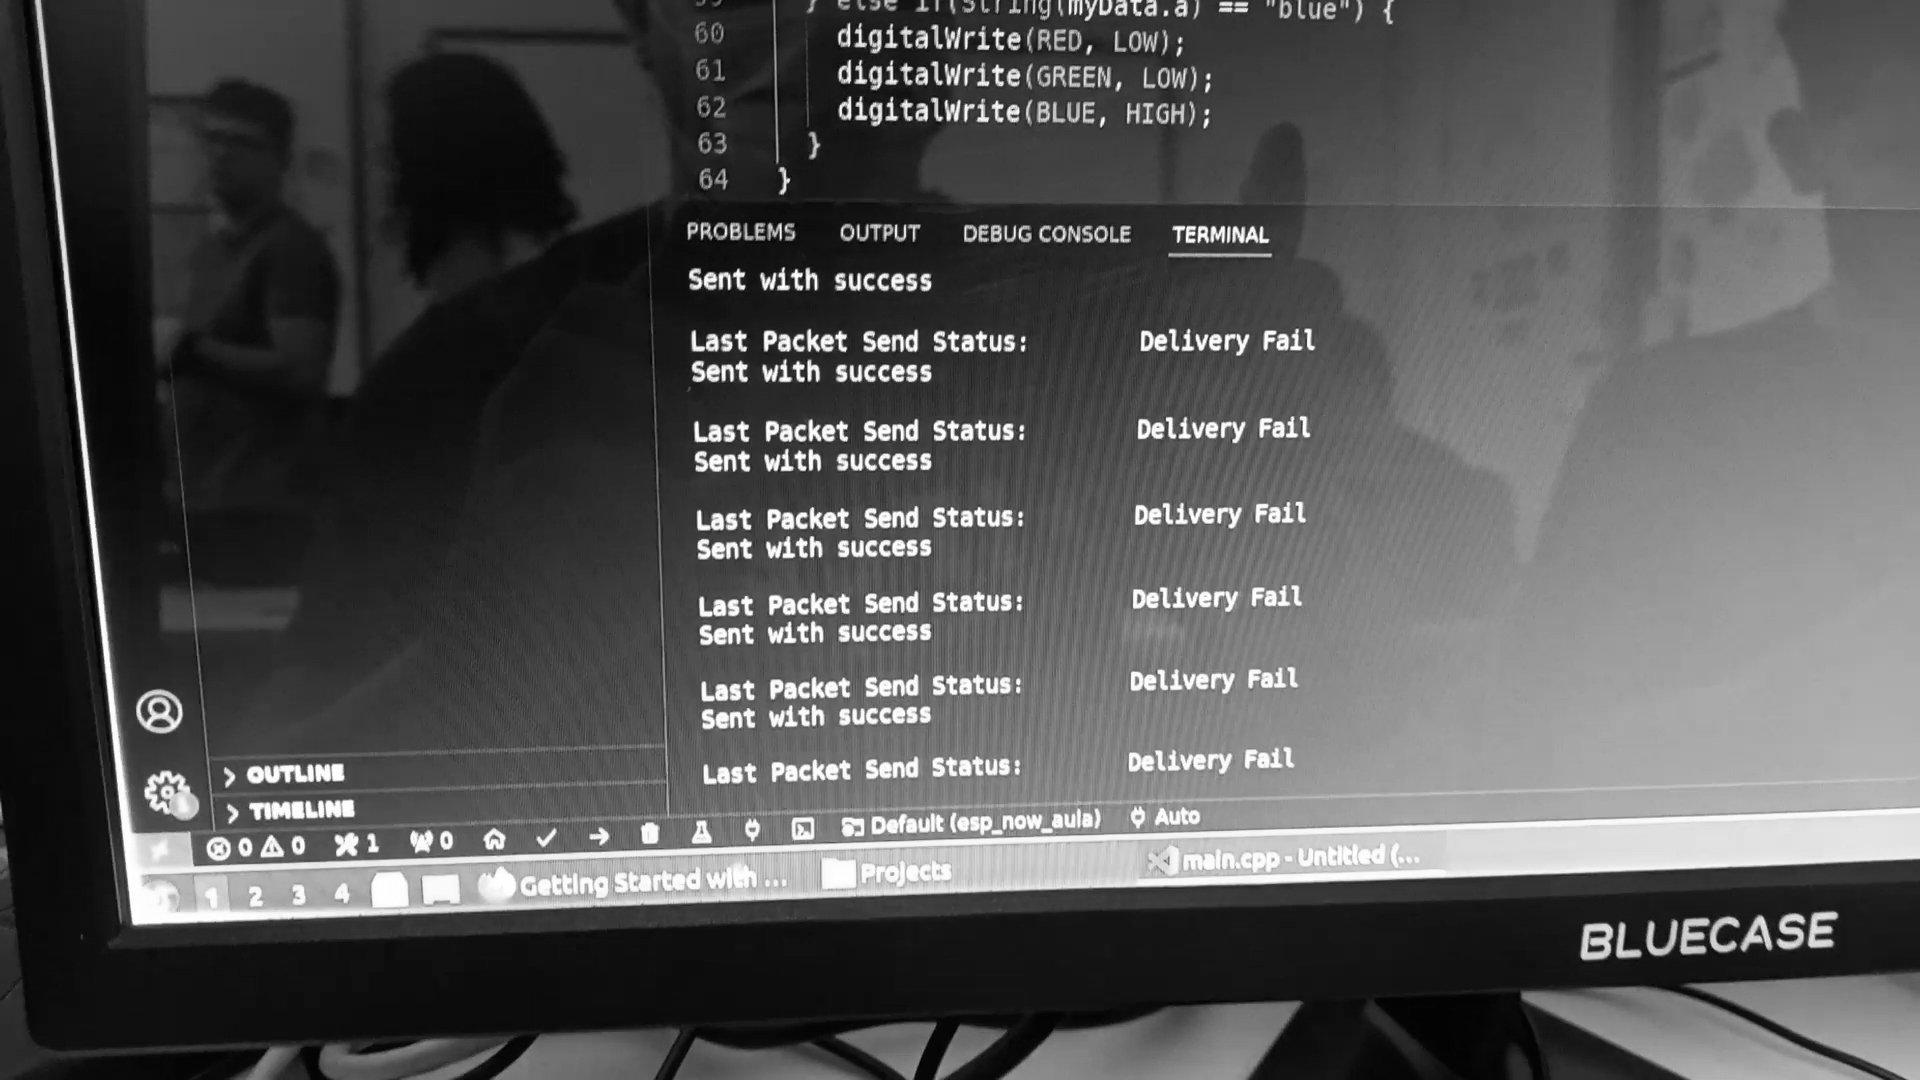
\includegraphics[width=0.5\linewidth]{img/20241202_091748.mp4_snapshot_00.08.622.jpg}
    \caption{Tela do monitor.}
    \label{fig:monitor}
\end{figure}

Um vídeo para conferir o resultado final está disponível no Youtube. Acesse por \href{https://youtu.be/Sk7I_T_a9ao}{aqui}.

\end{document}